\documentclass[a4paper]{article}



%% Language and font encodings
\usepackage[english]{babel}
\usepackage[utf8x]{inputenc}
\usepackage[T1]{fontenc}
\usepackage[compat=1.0.0]{tikz-feynman}
\usepackage{listings}


%% Sets page size and margins
\usepackage[a4paper,top=3cm,bottom=2cm,left=3cm,right=3cm,marginparwidth=1.75cm]{geometry}

%% Useful packages
\usepackage{amsfonts}
\usepackage{amsmath}
\usepackage{graphicx}
\graphicspath{ {./img/} }
\usepackage[colorlinks=true, allcolors=blue]{hyperref}
\usepackage{float}
\usepackage{enumerate}
\usepackage{subfig}

\title{REYES Nuclear Physics Mentoring Week 3}
\author{Aman Kumar}

\begin{document}
\maketitle
\section{Introduction}
This week's discussion began with the discussion on scattering amplitude. Scattering Amplitude $\mathbb{M}$ characterizes probability
of an interaction to occur.

$i\mathbb{M}\propto \langle final | \mathbb{S} -1 | initial \rangle$

Where $\mathbb{S}$ is known as S matrx. And we subtract 1 from the S matrix to remove identity which means the condition of no interaction
between the particles. \\

The S-matrix or scattering matrix relates the initial state and the final state of a physical system undergoing a scattering process.

\subsection{Scattering Theory}
Model independent features of scattering amplitudes are: 
\begin{enumerate}
    \item Spacetime Symmetry -Loretnz Invariance
    \item Internal Symmetry -Flavour,Baryon Number
    \item probability conservation -The S matrix is unnitary operator i.e $\mathbb{S}^{\dagger}\mathbb{S}=I$
    \item causality - Amplitudes are boundary values of analytic functions in complex energy plane.
    \item CPT Symmetry - Relates particle—anti-particles in scattering processes.
\end{enumerate}

\subsubsection{Probability Conservation}
The S matrix is unnitary operator i.e $\mathbb{S}^{\dagger}\mathbb{S}=I$.
After some work we can show that(in a limited energy region) $Im \mathbb{M} = \rho |\mathbb{M}|^2$.
\\
$\rho$ is known as phase space kinematic function. Characterizes on-shell scattering of two-particles.

\[
    \rho = \dfrac{\xi q^{\star}}{8\pi E^{\star}}
\]

also $q^{\star}=\dfrac{1}{2}\sqrt{E^{\star 2} - 4m^2}$ with $\xi = \begin{cases}
    \dfrac{1}{2} & identical \\
    1 & otherwise\\
\end{cases}$

\subsubsection{Phase Shift}
At a fixed energy, amplitude determined by magnitude and phase (2 real numbers). Therefore scattering amplitude, $\mathbb{M} = |\mathbb{M}|e^{i \delta}$

Imposing unitarity $Im \mathbb{M} = \rho |\mathbb{M}^{2}|$ we get $|\mathbb{M}| = \dfrac{1}{\rho} sin\delta$.
such that $\mathbb{M} = \dfrac{1}{\rho}e^{i \delta} sin \delta$ 

Here $\delta$ is the phase shift.

\subsubsection{K-Matrix}
We know that $Im \mathbb{M} = \rho|\mathbb{M}|^2$

This implies that $Im \mathbb{M}^{-1} = - \rho$ 
\\
$\implies \mathbb{M}^{-1} = K^{-1} - i \rho$
\\
$\mathbb{M} = K\dfrac{1}{1=i\rho K}$

Note: K matrix can be related to phase shift by $K = \rho cot \delta$


\section{Exercises}
\subsection{ Exercise 1}
\textbf{Plot $\rho$(phase space) for identical particles in the range $1.8 \leq \dfrac{E*}{m} \leq 3.2$}
\\ \\ \\ \\
\textbf{Solution:}\\
\\
$\rho = \dfrac{\xi q^{\star}}{8 \pi E^{\star}}$ 
\\
\\
For identical particles : $\xi = 1/2$ 
\\
\\
and $q^{\star}=\dfrac{1}{2}\sqrt{E^{\star 2} - 4m^2}$
\\
\\
\\
This makes it $\rho = \dfrac{1}{32 \pi} \dfrac{\sqrt{ E^{\star} - 4m^2 }}{ E^{\star}}$
\\
\\
\\
$\rho = \dfrac{1}{32 \pi} \sqrt{1 - 4(\dfrac{m}{E^{\star}})^2}$
\\
\\
\\
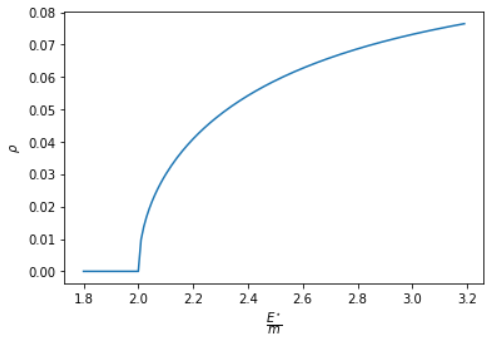
\includegraphics{ex1.png}

\begin{lstlisting}[label=code-used,caption=Code used]
import matplotlib.pyplot as plot
import numpy as np 
import cmath as cm 

def f(x):
    return (1/32*cm.pi)*cm.sqrt(1 - (4*x**(-2)))

f = np.vectorize(f)
x = np.arange(1.8,3.2,0.01)
y = f(x)
plt.plot(x,np.real(y))
plt.xlabel(r'$\dfrac{E^{\star}}{m}$')
plt.ylabel(r'$\rho$')
\end{lstlisting}


\subsection{Exercise 2}
\textbf{Derive the phase shift representation for the scattering amplitude.}
\\ \\ \\
We know that $\mathbb{M} = |\mathbb{M}|e^{i\delta}$, using euler's formula, can be expanded as \[ \mathbb{M} = |\mathbb{M}|(cos \delta  + i sin \delta) \].
\\ \\ 
We also know that \[ Im \mathbb{M} = \rho |\mathbb{M}|^2 ]\]

So from the above two relations we get that 
\[
    |\mathbb{M}| sin \delta = \rho |\mathbb{M}|^2
    \implies   \rho = \dfrac{sin \delta}{|\mathbb{M}|} 
\] 
\\ \\
Substituting $\mathbb{M} = |\mathbb{M}|e^{i\delta}$ in the above result we get: 
\[
    \mathbb{M} = \dfrac{1}{\rho}e^{i\delta}sin \delta
\]
\subsection{Exercise 3}
\textbf{Show that $ Im \mathbb{M}^{-1} = -\rho$}
\\ \\ \\ \\
Ww know that $\mathbb{M} = |\mathbb{M}|e^{i\delta}$.\\ \\ \\Right multiplication by $\mathbb{M}^{-1}$.
\[
    \mathbb{M} \mathbb{M}^{-1} = e^{i \delta} |\mathbb{M}|\mathbb{M}^{-1} = I
\]
\[
    \implies \mathbb{M}^{-1} = \dfrac{I}{e^{i\delta}|\mathbb{M}|} = \dfrac{1}{e^{i\delta|\mathbb{M}|}} = 
    \dfrac{e^{-i\delta}}{|\mathbb{M}|}
\]
\[
    \mathbb{M}^{-1} =\dfrac{e^{-i\delta}}{|\mathbb{M}|} = \dfrac{cos(-\delta) + i sin(-\delta) }{|\mathbb{M}|} =
    \dfrac{\rho (cos \delta - i sin \delta)}{sin \delta} \implies Im \mathbb{M}^{-1} = - \rho
\]


\subsection{Exercise 4}
\textbf{Show that $K^{-1} = \rho cot \delta$}
\\ \\ \\ \\
\[
    \mathbb{M}^{-1} = \dfrac{\rho cos \delta -  i \rho sin \delta}{sin \delta} = K^{-1} - \rho i
    \\ \\
    \implies K^{-1} = \dfrac{\rho cos \delta}{sin \delta} = \rho cot \delta
\]


\end{document}